\documentclass[a4paper,11pt,oneside]{article}
\usepackage{header}
% PLECS version noch rein
\begin{document}
\pagestyle{fancy}
\fancyhf{}
\fancyhead[L]{Kurzanleitung STM32-Programmierung in PLECS}
\section*{Kurzanleitung STM32-Programmierung in PLECS}
In PLECS simulierte Steuerungen oder Regelungen können mit STM32-Blöcken erweitert werden, um die Peripherie des Mikrocontrollers anzusteuern. Danach kann Code für den µC in PLECS generiert, kompiliert und hochgeladen werden. Anschließend können im sog. \enquote{External Mode} während der Programmausführung Variablen aus dem µC gesetzt und in PLECS-Scopes angezeigt werden. \\ 
Diese Kurzanleitung orientiert sich an der Dokumentation \enquote{\href{https://www.plexim.com/sites/default/files/stm32manual.pdf}{STM32 Target Support User Manual - Ver. 1.4}\footnote{\url{https://www.plexim.com/sites/default/files/stm32manual.pdf}}} von PLECS; nachfolgend bezeichnet als \enquote{TSU-Manual}. An einigen Stellen wird darauf verwiesen. Die referenzierte Version der Dokumentation ist diesem Dokument angehängt. Zur einfacheren Erklärung wird eine bereits für den STM32G474 vorkonfigurierte PLECS-Simulation genutzt. Diese ist dem Dokument beigefügt. Die Simulation wurde erstellt und getestet mit PLECS Version 4.8.2 und dem STM32 Target Support Package Version 1.4.3.
\subsection*{Installation des Target Support Package}
Um die STM32-Codegenerierung nutzen zu können, muss \enquote{PLECS Coder} installiert sein. Die Installation des Target Support Package ist auf S. 3 \enquote{Installing the Target Support Package} des TSU-Manual beschrieben. 
\subsection*{Konfigurieren des Targets}
Die beigefügte Simulation ist bereits für den STM32G474 mit Beschaltung auf einem Nucelo-Board konfiguriert. PLECS unterstützt aber auch die µCs: STM32G431, STM32F334 und STM32F303. Für diese müssen unter \textbf{Coder > Coder options... > Target} die entsprechenden Parameter eingestellt werden.
\subsection*{PLECS-Simulationen für Ausführung auf µC adaptieren}
In der beigefügten Simulation wird ein 1Hz Rechtecksignal auf der internen LED des Nucleo-Boards ausgeben, sowie ein sinusmoduliertes PWM-Signal, welches über den blauen Taster auf dem Board abgeschaltet werden kann. Es ist zu erkennen, dass die Signalgenerierung und Logik weiterhin aus normalen PLECS-Blöcken besteht. Lediglich die Ansteuerung der Schnittstellen des µCs wird mit Blöcken der \enquote{STM 32 Target} PLECS-Library realisiert. Dadurch ist es möglich große Teile aus bereits vorhandenen Simulationen beizubehalten und schnell für die Ausführung auf externer Hardware zu adaptieren. Eine Beschreibung aller Blöcke der Library findet sich im TSU-Manual ab S. 31. In den meisten Blöcken müssen Ein- bzw. Ausgangspins definiert werden. Es können nur Pins verwendet werden, die auch intern mit der entsprechenden Peripherie verbunden sind. Die Belegung ist dem Datenblatt des jeweiligen µCs zu entnehmen.
\subsection*{Code generieren, kompilieren und hochladen}
\label{Codegenerieren}
Um den Code auf einem Nucleo-Board oder mit Hilfe eines ST-Link Progammers hochzuladen, muss unter \textbf{Coder > Coder options... > Target > Programming Interface: \enquote{OpenOCD}}, sowie unter \textbf{... > Build Type \enquote{Build and Program}} ausgewählt sein. Mit einem Klick auf \textbf{Build} kann der Prozess gestartet werden. Der generierte Code und die kompilierten Binaries werden im Simulationszverzeichnis abgelegt. Hilfreich für die Verdrahtung: Mit der Option \textbf{\enquote{Generate Pinmap File}} kann zusätzlich eine Grafik der Pinbelegung erzeugt werden.
\subsection*{External Mode}
Im External Mode können während der Progammausführung Variablen aus dem µC gesetzt und in PLECS-Scopes angezeigt werden. PLECS konfiguriert eine Schnittstelle im Code und tauscht die Daten über den UART Bus oder JTAG aus. Für die Verwendung über den UART Bus muss der µC per USB verbunden sein. (Unter \textbf{Coder > Coder options... > Target > External Mode > External mode: \enquote{Serial}} auswählen.) Mit den restlichen Optionen können die Buffergröße und die Pins, die für die Datenübertragung verwendet werden sollen, eingestellt werden. Standardmäßig ist der UART ausgewählt, welcher auf dem Nucleo Board mit dem USB verbunden ist. Sollen bestimmte Größen zur Laufzeit verändert werden können, so müssen die entsprechenden Blöcke, welche die Größen enthalten unter \textbf{Coder > Coder options... > Parameter Inlining} per Drag and Drop hinzugefügt werden. Jetzt muss der µC neu geflasht werden (siehe \nameref{Codegenerieren}). Läuft der entsprechende Code auf dem µC, kann sich unter \textbf{Coder > Coder options... > External Mode > Target Device} mit dem Controller verbunden werden. In den Scopes werden nun live die Werte der enstprechenden Variablen im µC angezeigt. Optionen zu Triggering und Sampling der Scopes befinden sich im oben genannten Menü. Die Übertragung der Werte dauert immer einige Sekunden. Die zur Änderung konfigurierten Größen können wie gewohnt in den Blöcken geändert werden.
Wird der External Mode nicht mehr benötigt, sollte er deaktiviert und der µC neu geflasht werden, da sonst das Programm unnötig verlangsamt werden kann.
\subsection*{Häufige Fehlermeldungen}
\textit{\textbf{Fehlermeldung:}} Trouble precision floating point format not supported. Please change the setting on the 'General' tab of the 'Coder options' dialog to 'float'.\\
\textit{\textbf{Lösung:}} \textbf{Coder > Coder options... > General > Floating point format: \enquote{float}}
\\\\
\textit{\textbf{Fehlermeldung:}} Verschiedene Fehlermeldungen zu control task execution rate, discretization step size oder base step size. \\
\textit{\textbf{Lösung: }}\textbf{Coder > Coder options... > Scheduling > Discretization step size} verkleinern oder vergrößern, je nach Fehlermeldung.
\\\\
\textit{\textbf{Fehlermeldung:}} Invalid or unsupported function for pin XX. \\
\textit{\textbf{Lösung:}} Ein Pin unterstützt die geforderte Funktion (z.B. PWM) nicht. Im entsprechenden Block die Pinbelegung ändern. Mögliche Pins werden meist in der Fehlermeldung angezeigt.
\\\\\\
\today \\
Capstone Gruppe Prof. Dick, Sommersemester 2024\\
Bei Fragen: \href{mailto:moritz@prenzlow.de}{moritz@prenzlow.de}\\
\newpage
\section*{Anhang}
\newpage
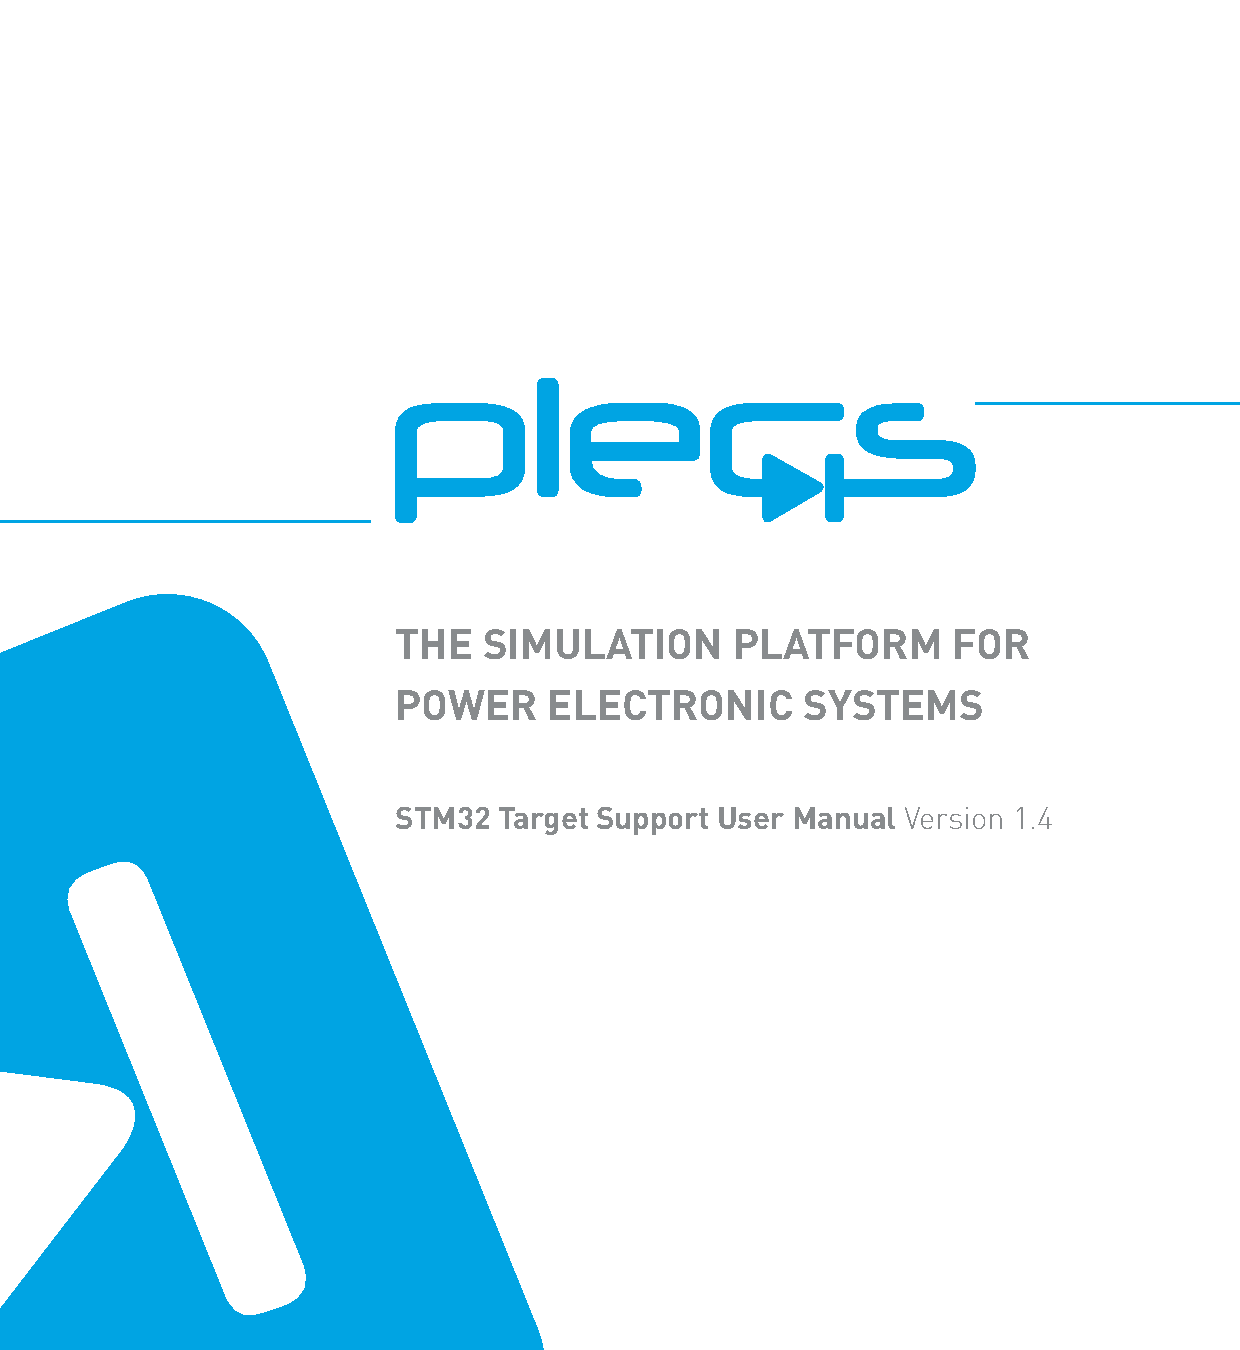
\includepdf[pages=-]{stm32manual.pdf}
\printbibliography
\end{document}